\begin{enumerate}
\item In \figref{fig:circ}, from an external point $P$, two tangent $PQ$ and $PR$ are drawn to a circle of radius $4cm$ with center $O$. If$\angle{PQR}=90\degree$, then length of $PQ$ is \underline {\hspace{4cm}}.
\begin{enumerate}[label=(\alph*)]
\item $3cm$ 
\item $4cm$
\item $2cm$
\item $2{\sqrt{2}}cm$ 
\end{enumerate}
\begin{figure}[H]
\centering
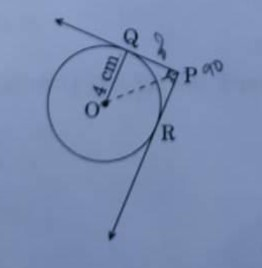
\includegraphics[width=\columnwidth]{figs/circ.jpg}
\caption{}
\label{fig:circ}
\end{figure}
\item In \figref{fig:circ2}, $PQ$ is tangent to the circe with center at $O$, at the point $B$. If$\angle AOB=100\degree$, then$\angle ABP$ is equal to\newline
\begin{enumerate}[label=(\alph*)] 
\item $50\degree$ 
\item $40\degree$ 
\item $60\degree$ 
\item $80\degree$
\end{enumerate}
\begin{figure}[H]
\centering
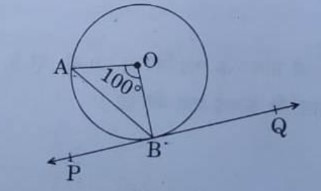
\includegraphics[width=\columnwidth]{figs/circ2.jpg}
\caption{}
\label{fig:circ2}
\end{figure}
\item In \figref{fig:circ3}, quadrilateral $ABCD$ is drawn to circumscribe a circle. Prove that\newline
$AB+CD=BC+AD$
\begin{figure}[H]
\centering
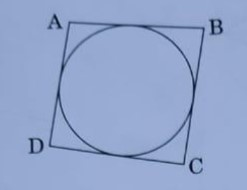
\includegraphics[width=\columnwidth]{figs/circ3.jpg}
\caption{}
\label{fig:circ3}
\end{figure}
\item In \figref{fig:circ4}, find the perimeter of $\triangle ABC$, if $AP=12cm$
\begin{figure}[H]
\centering
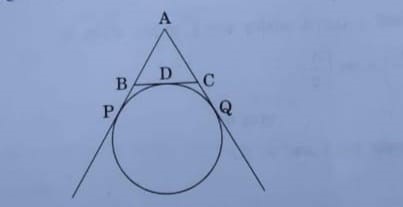
\includegraphics[width=\columnwidth]{figs/circ4.jpg}
\caption{} 
\label{fig:circ4}
\end{figure}
\end{enumerate}
